% !TeX encoding = UTF-8

\documentclass{protokol}

\usepackage{tikz}
\usetikzlibrary{calc}
\usetikzlibrary{arrows}

%====== Units =====
\usepackage{siunitx}
\sisetup{inter-unit-product =\ensuremath{\cdot}}
\sisetup{group-digits = integer}
\sisetup{output-decimal-marker = {,}}
\sisetup{exponent-product = \ensuremath{\cdot}}
\sisetup{separate-uncertainty}
\sisetup{tight-spacing = false}
%\sisetup{scientific-notation = true}
%\sisetup{round-mode=places,round-precision=4}
%\sisetup{evaluate-expression}


%====== Grafy =====
\usepackage{pgfplots}
\pgfplotsset{width=0.8\linewidth, compat=1.17}
\def\plotcscale{0.8}
\usepackage{pgfplotstable}
\usepackage[figurename=Graf]{caption} % figure caption rename
%====== Rovnice align block ======
\usepackage{amsmath}
\setlength{\jot}{10pt} % rozestup mezi řádky

\graphicspath{ {./img/} }

%====== Vyplňte údaje ======
\jmeno{Jakub Charvot}
\kod{240844}
\rocnik{2.}
\obor{MET}
\skupina{MET/4}
\spolupracoval{Radek Kučera}

\merenodne{10.\,11.\,2022}
\odevzdanodne{24.\,11.\,2022}
\nazev{Operační usměrňovače}
\cislo{4} %měřené úlohy

\predmet{Analogové elektronické obvody}
\ustav{Ústav mikroelektroniky}
\skola{FEKT VUT v Brně}

\def\para{x+0}
\def\parb{\para-80}

% CSV
\usepackage{blindtext}

\usepackage{subfiles} % Best loaded last in the preamble
\usepackage{datatool}

\DTLloaddb[omitlines=2]{prvni}{data/prvni-cast.csv}
\DTLloaddb[omitlines=2]{druha}{data/druha-cast.csv}



\begin{document}
	%====== Vygenerování tabulky ======
%	\maketitle
	%====== Úvodní texty protokolu ======

%	\section{Teoretický úvod}
%		\begin{figure}[h!]
    \centering
    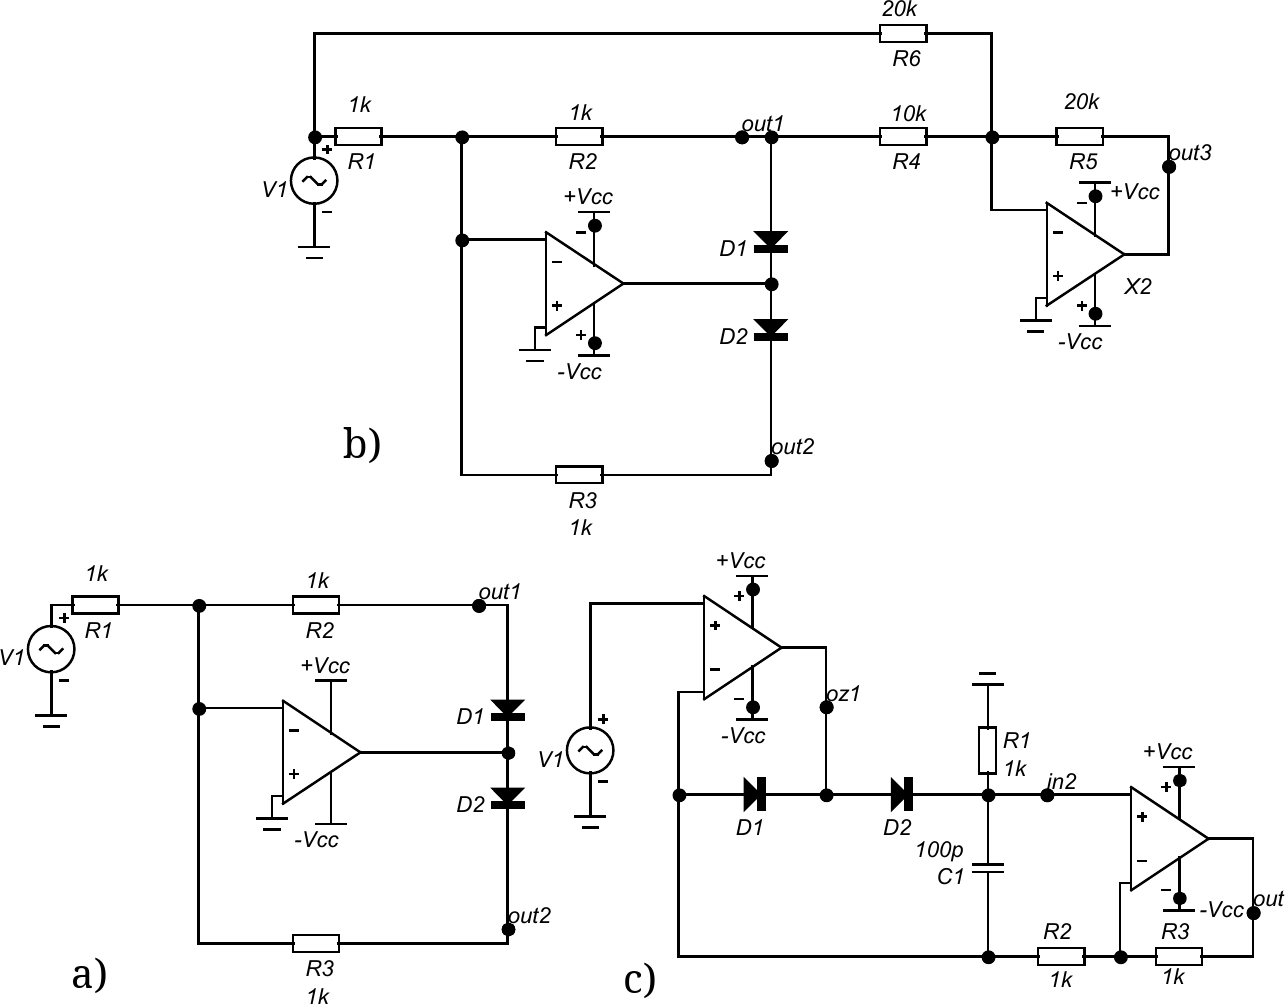
\includegraphics[width=\textwidth]{schema.png}
    \centering
    \caption{Schémata zapojení -- a) jednocestný usměrňovač, b) dvoucestný usměrňovač, c) dvoucestný usměrňovač s minimem přesných součástek.}
    \label{fig:schema}
\end{figure}



\subsection{Funkce jednotlivých zapojení}

    Operační zesilovač s OZ má za úkol překonat nedostatky, které má zapojení pouze s diodami, které díky svému prahovému napětí nedokáží usměrňovat velmi malá napětí. 
    
    Zapojení 1a) je jednocestný usměrňovač, kdy je vždy přes jednu diodu uzavřená záporná zpětná vazba a druhá dioda je uzavřená. Na výstupu je pak signál jednocestně usměrněný a invertovaný. 
    
    Zapojení 1b) pak tento signál zdvojnásobí a sečte s původním vstupním signálem, ve výsledku tedy původní záporné půlvlny zůstanou a kladné po sečtení odpovídají opět záporným. Výsledkem je tedy dvoucestně usměrněný invertovaný signál. 
    Nevýhodou tohoto zapojení je nutnost použít dva co nejshodnější odpory a k nim jeden, který odpovídá hodnotu přesně polovině, při nedodržení nebudou na výstupu půlvlny stejně velké, toto značně zdražuje zapojení. 

    Tento problém se snaží řešit zapojení 1c), kdy pro správnou funkci stačí jedna dvojice přesných odporů \( R_2\) a \(R_3\). Záporná zpětná vazba prvního OZ je vždy uzavřena přes druhý OZ, díky diodám je ale cesta zpětné vazby jiná pro kladný a pro záporný signál, takže ve výsledku je na výstupu druhého OZ signál vždy kladný, neboli dvoucestně usměrněný.   
%		
%	% \newpage
%	\section{Výsledky počítačové simulace}
%		\begin{figure}[h!]
    \centering
    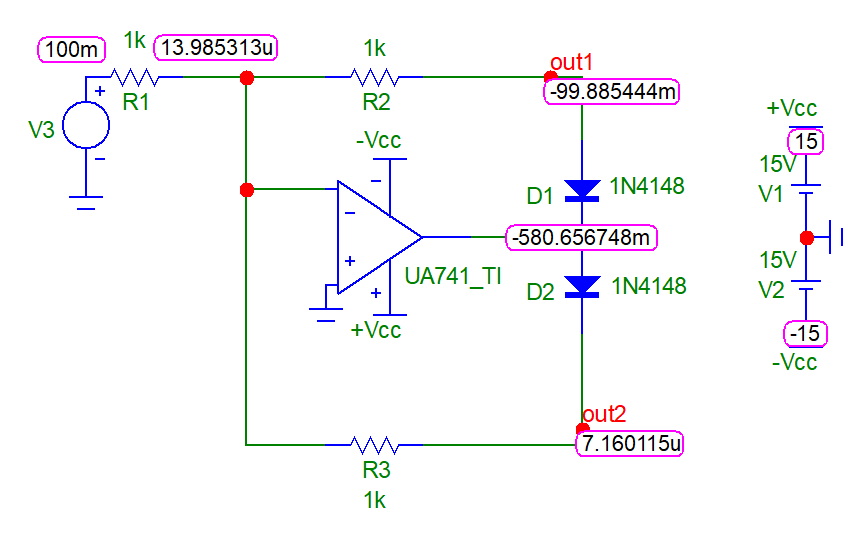
\includegraphics[width=0.63\textwidth]{microcap/1-dcbod.png}
    \caption{Zapojení a) -- stejnosměrný prac. bod pro kladné vstupní napětí.}
    \label{fig:microcap/.png}
\end{figure}

\begin{figure}[h!]
    \centering
    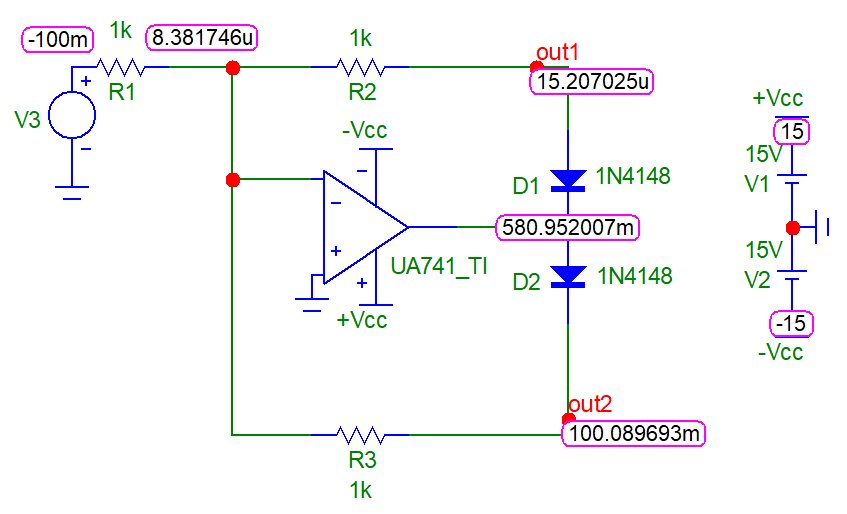
\includegraphics[width=0.63\textwidth]{microcap/1-dcbod2.png}
    \caption{Zapojení a) -- stejnosměrný prac. bod pro záporné vstupní napětí.}
    \label{fig:microcap/.png}
\end{figure}

\begin{figure}[h!]
    \centering
    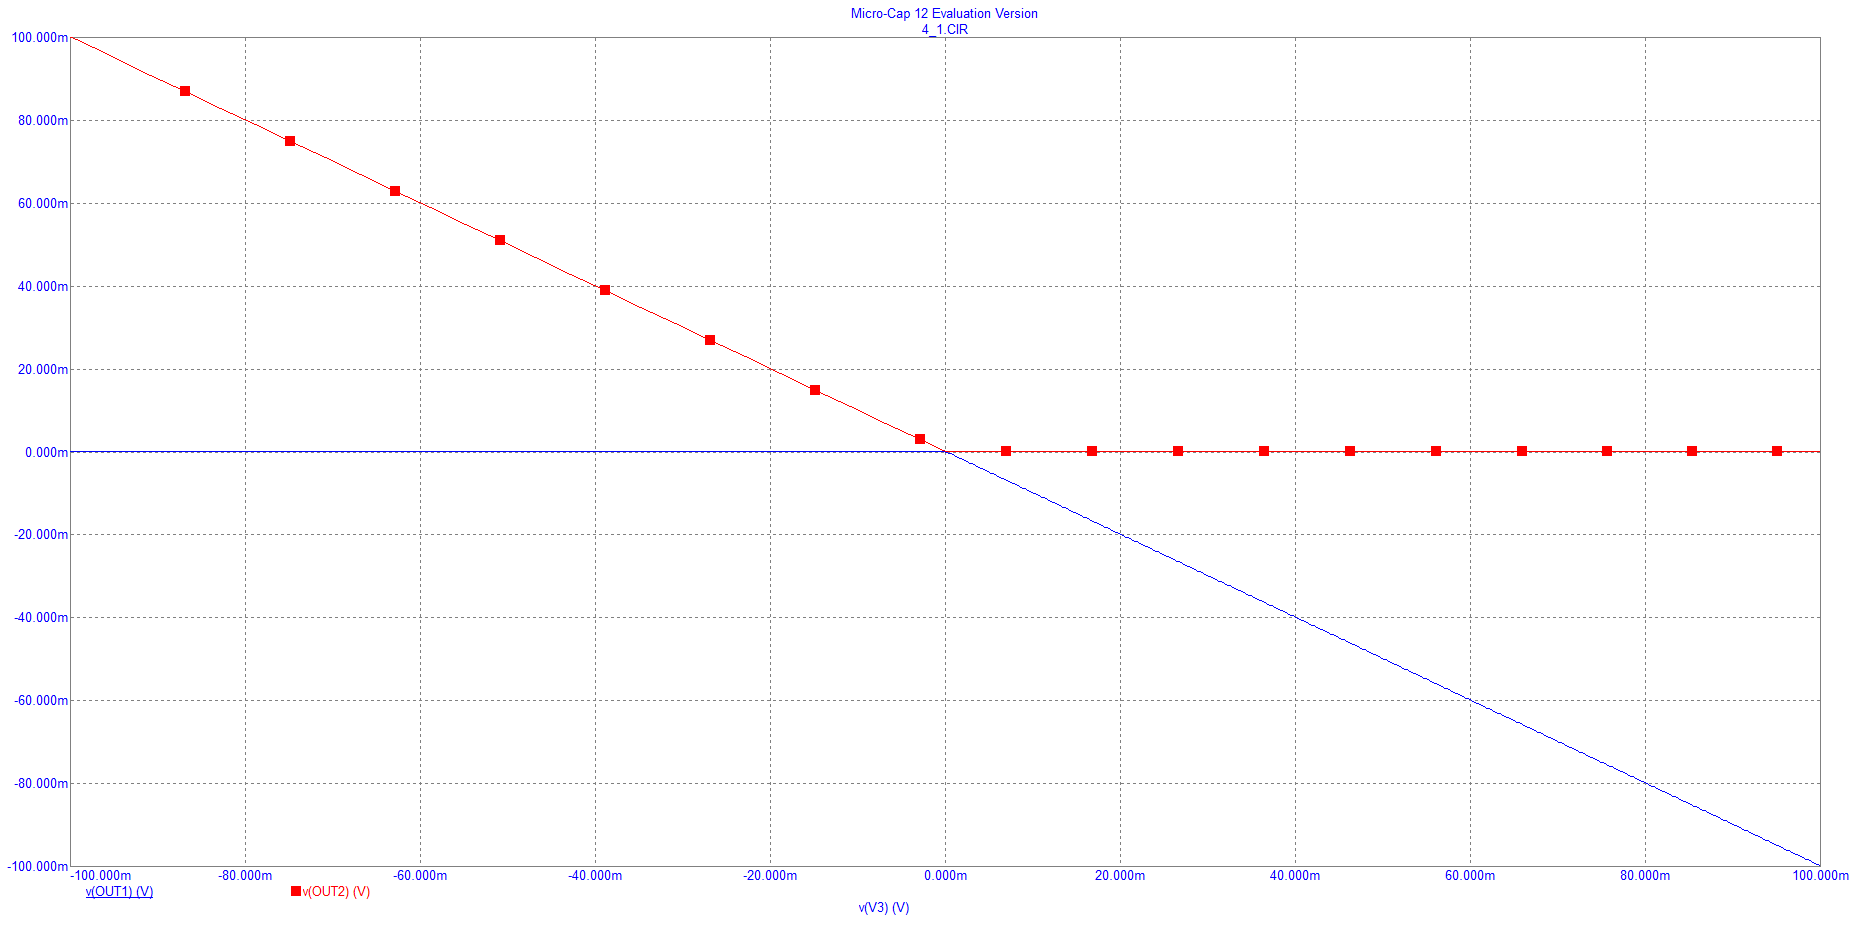
\includegraphics[width=0.8\textwidth]{microcap/1-dcprevodni.png}
    \caption{Zapojení a) -- stejnosměrná převodní charakteristika.}
    \label{fig:microcap/.png}
\end{figure}

\begin{figure}[h!]
    \centering
    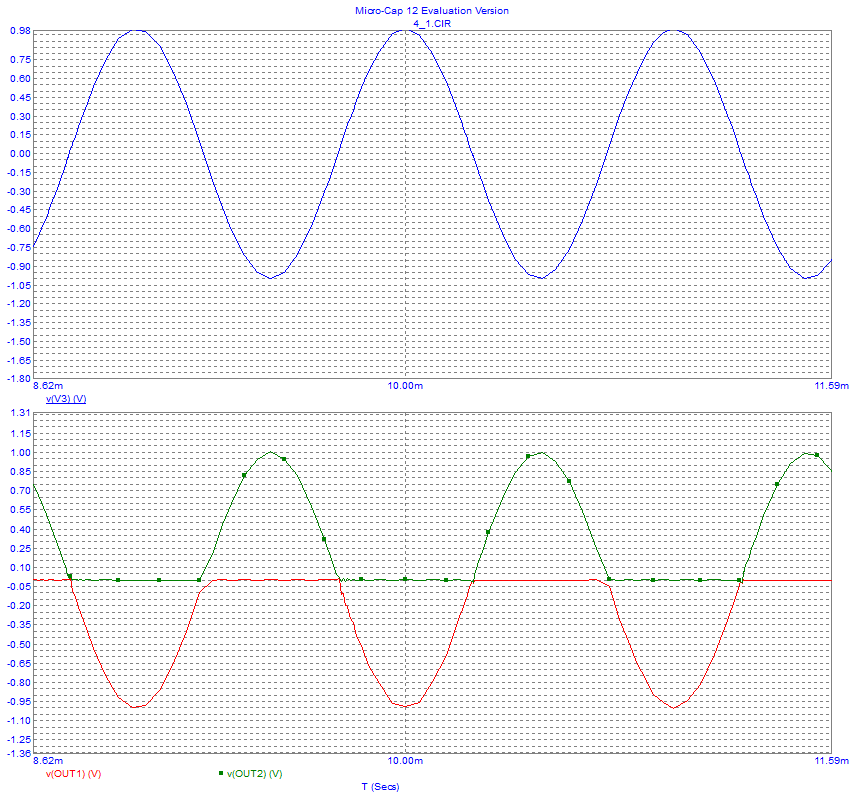
\includegraphics[width=0.8\textwidth]{microcap/1-transient-1khz-1v.png}
    \caption{Zapojení a) -- časová závislost obou výstupních napětí na vstupním napětí, jednocestné zesílení, \(f=\qty{1}{\kilo\hertz}, U_M=\qty{1}{\volt}\).}
    \label{fig:microcap/.png}
\end{figure}

\begin{figure}[h!]
    \centering
    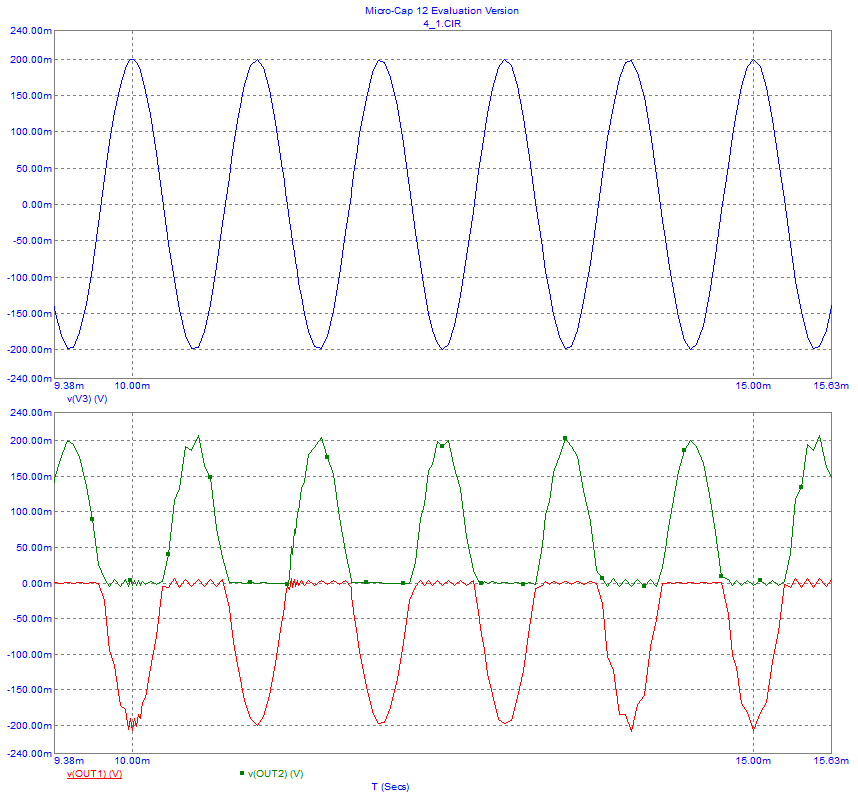
\includegraphics[width=0.7\textwidth]{microcap/1-transient-1khz-0.2v.png}
    \caption{Zapojení a) -- časová závislost obou výstupních napětí na vstupním napětí, nejmenší amplituda, při které zapojení obstojně usměrňuje, \(f=\qty{1}{\kilo\hertz}, U_M=\qty{200}{\milli\volt}\).}
    \label{fig:microcap/.png}
\end{figure}

\begin{figure}[h!]
    \centering
    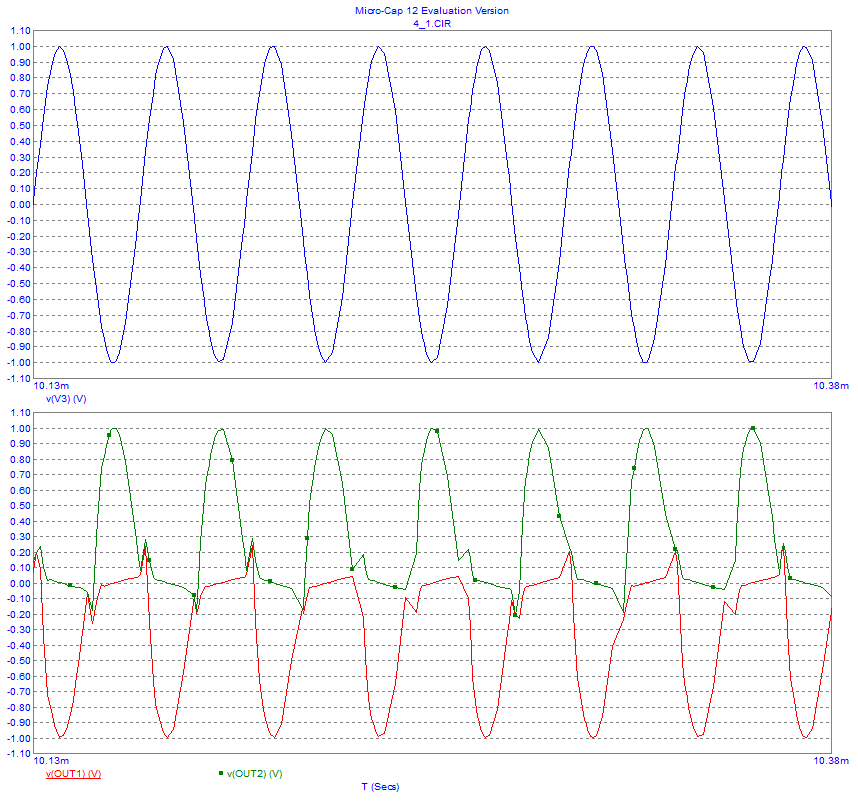
\includegraphics[width=0.7\textwidth]{microcap/1-transient-30khz-1v.png}
    \caption{Zapojení a) -- časová závislost obou výstupních napětí na vstupním napětí, nejvyšší frekvence, při které zapojení obstojně usměrňuje, \(f=\qty{30}{\kilo\hertz}, U_M=\qty{1}{\volt}\).}
    \label{fig:microcap/.png}
\end{figure}

\begin{figure}[h!]
    \centering
    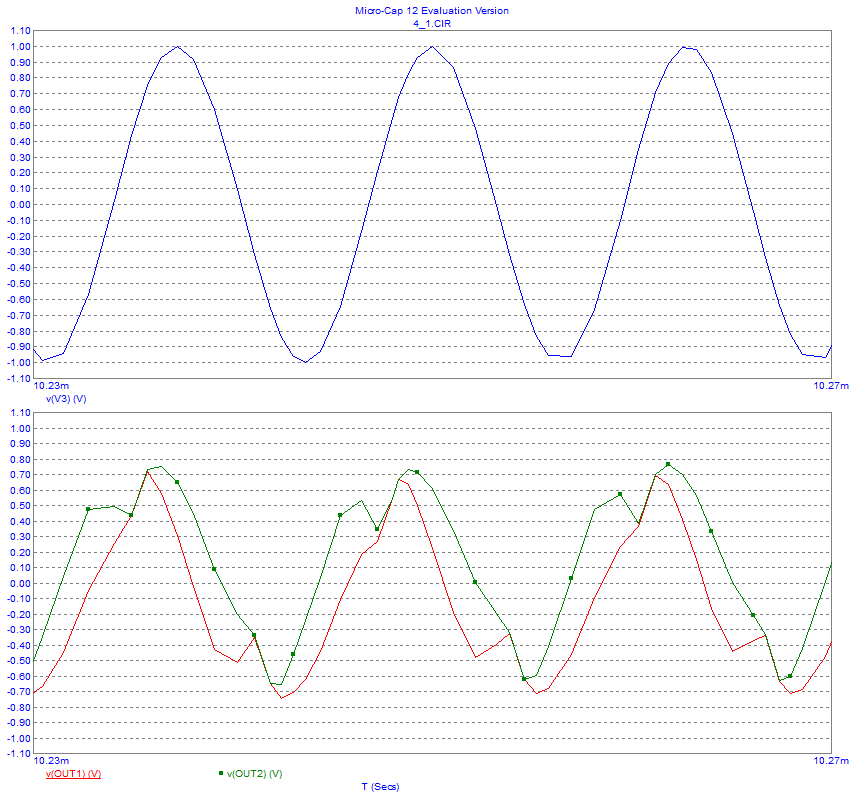
\includegraphics[width=0.8\textwidth]{microcap/1-transient-100khz-1v.png}
    \caption{Zapojení a) -- časová závislost obou výstupních napětí na vstupním napětí, příliš vysoká frekvence, k usměrnění nedochází vůbec, \(f=\qty{100}{\kilo\hertz}, U_M=\qty{1}{\volt}\).}
    \label{fig:microcap/.png}
\end{figure}    

% \begin{figure}[h!]
%     \centering
%     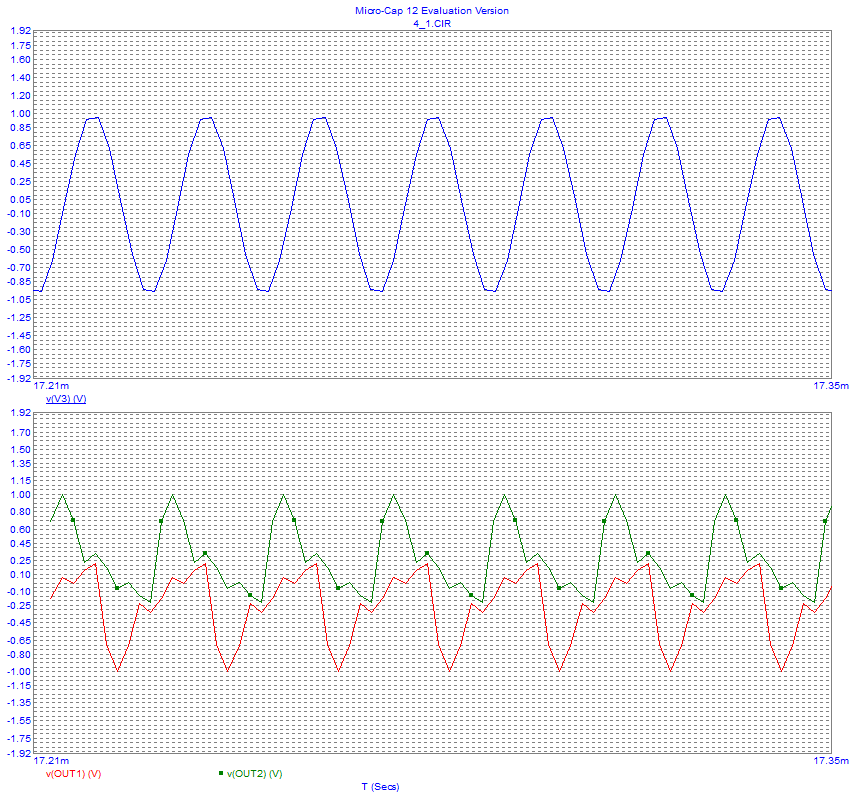
\includegraphics[width=0.8\textwidth]{microcap/1-transient-50khz-1v.png}
%     \caption{microcap/.png}
%     \label{fig:microcap/.png}
% \end{figure}

\begin{figure}[h!]
    \centering
    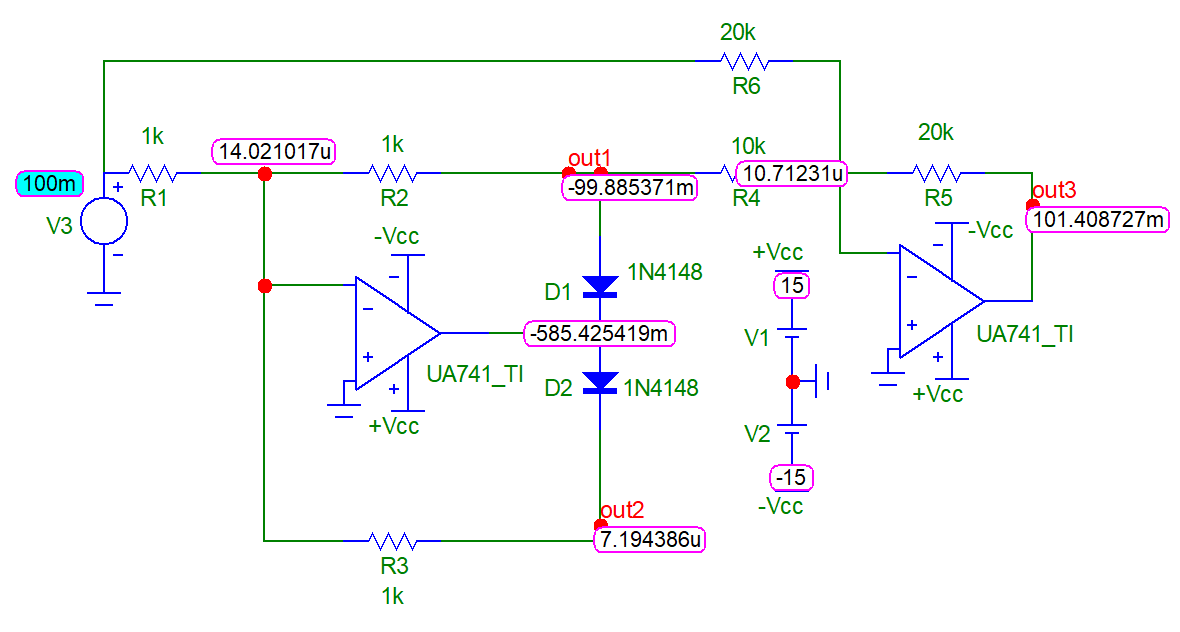
\includegraphics[width=0.8\textwidth]{microcap/2-dcbod.png}
    \caption{Zapojení b) -- stejnosměrný prac. bod při kladném napětí na vstupu, na výstupu kladné napětí.}
    \label{fig:microcap/.png}
\end{figure}

\begin{figure}[h!]
    \centering
    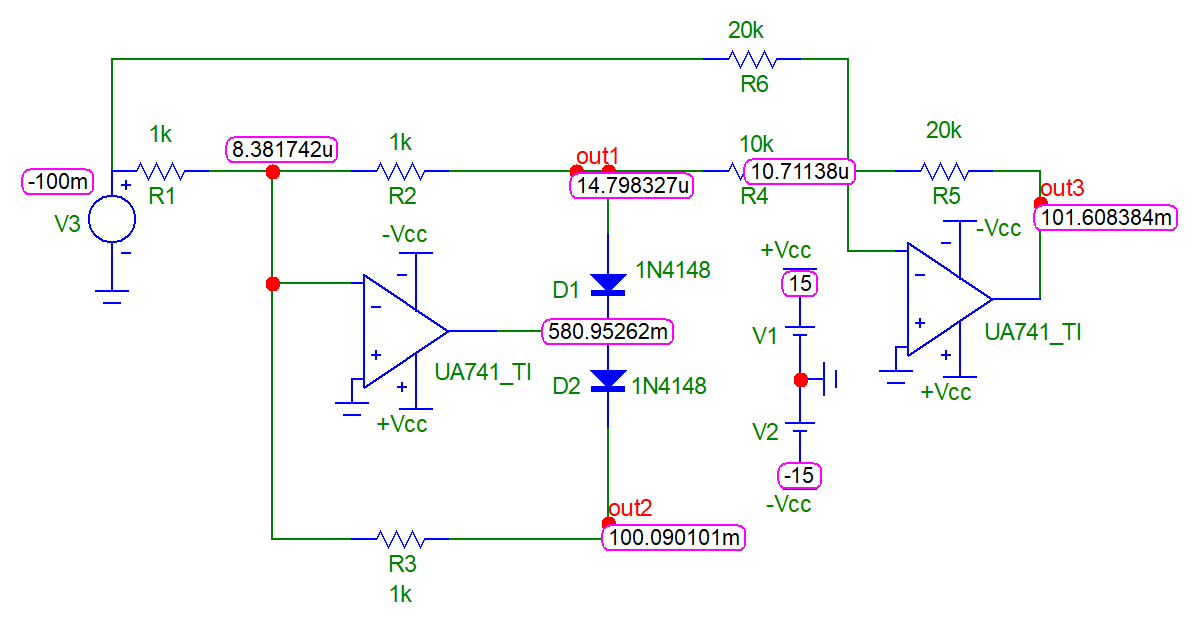
\includegraphics[width=0.61\textwidth]{microcap/2-dcbod2.png}
    \caption{Zapojení b) -- stejnosměrný prac. bod při záporném napětí na vstupu, na výstupu opět kladné napětí.}
    \label{fig:microcap/.png}
\end{figure}

\begin{figure}[h!]
    \centering
    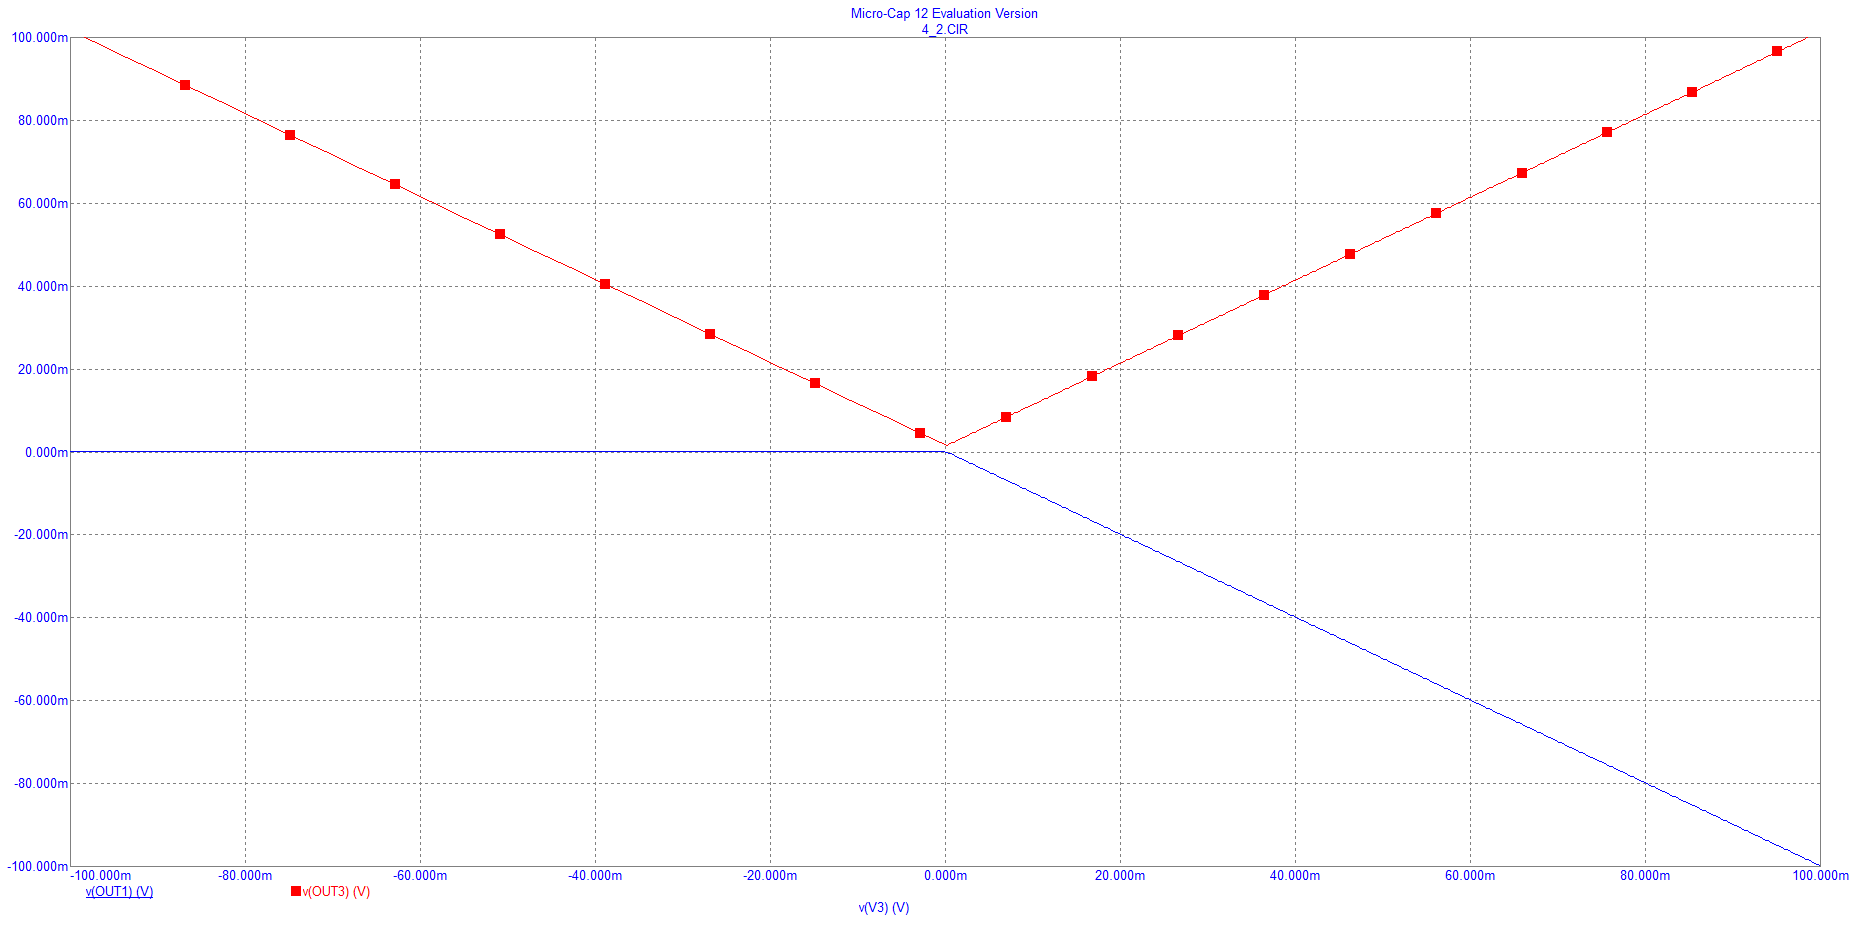
\includegraphics[width=0.61\textwidth]{microcap/2-dcprevodni.png}
    \caption{Zapojení b) -- stejnosměrná převodní charakteristika dvoucestného usměrnění.}
    \label{fig:microcap/.png}
\end{figure}

\begin{figure}[h!]
    \centering
    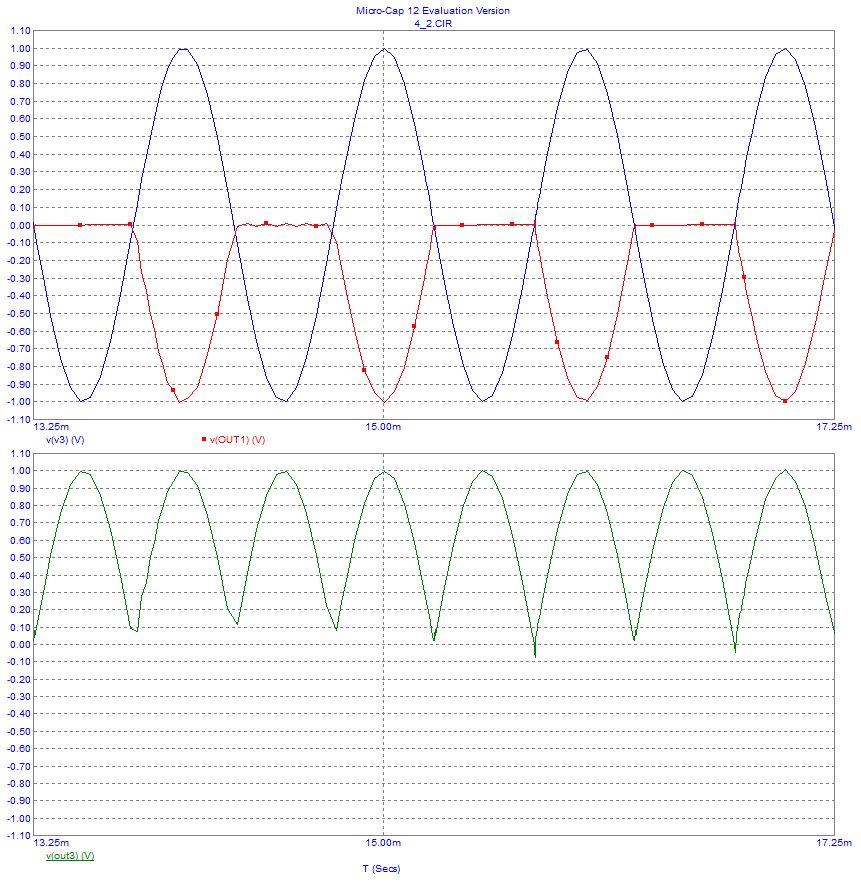
\includegraphics[width=0.61\textwidth]{microcap/2-transient-1khz-1v.png}
    \caption{Zapojení b) -- časová závislost napětí na výstupech obou OZ na vstupním napětí, jednocestné a dvoucestné usměrnění, \(f=\qty{1}{\kilo\hertz}, U_M=\qty{1}{\volt}\).}
    \label{fig:microcap/.png}
\end{figure}

% \begin{figure}[h!]
%     \centering
%     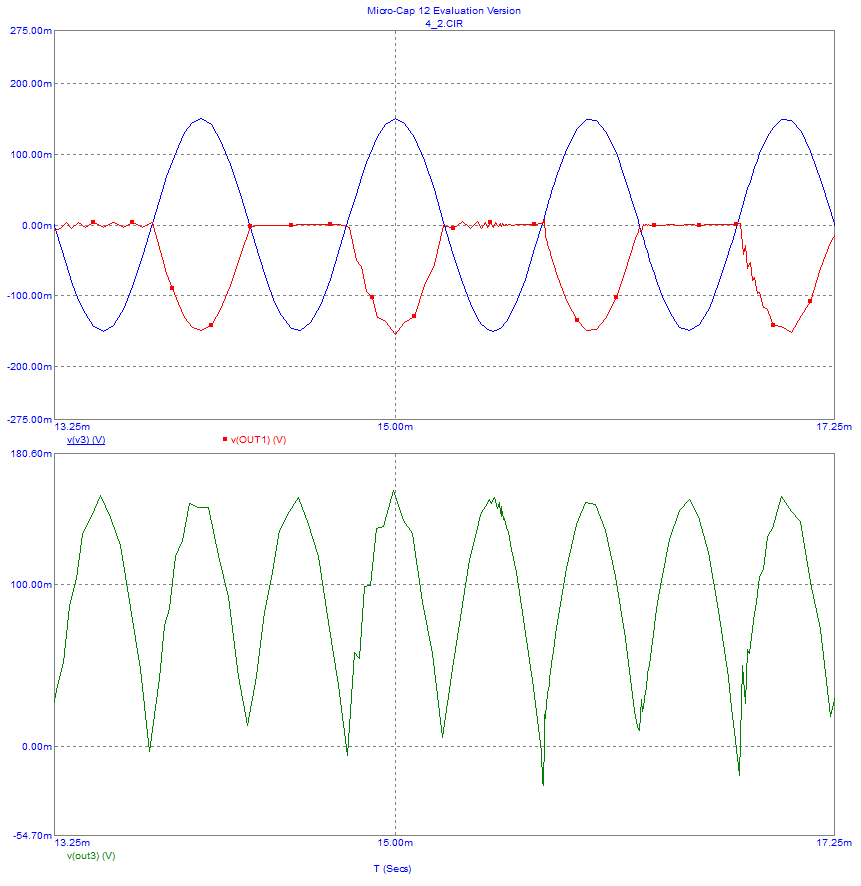
\includegraphics[width=0.8\textwidth]{microcap/2-transient-1khz-0.15v.png}
%     \caption{Zapojení b) -- časová závislost napětí na výstupech obou OZ na vstupním napětí, nejmenší amplituda, při které uspokojivě usměrňuje, \(f=\qty{1}{\kilo\hertz}, U_M=\qty{150}{\milli\volt}\).}
%     \label{fig:microcap/.png}
% \end{figure}

\begin{figure}[h!]
    \centering
    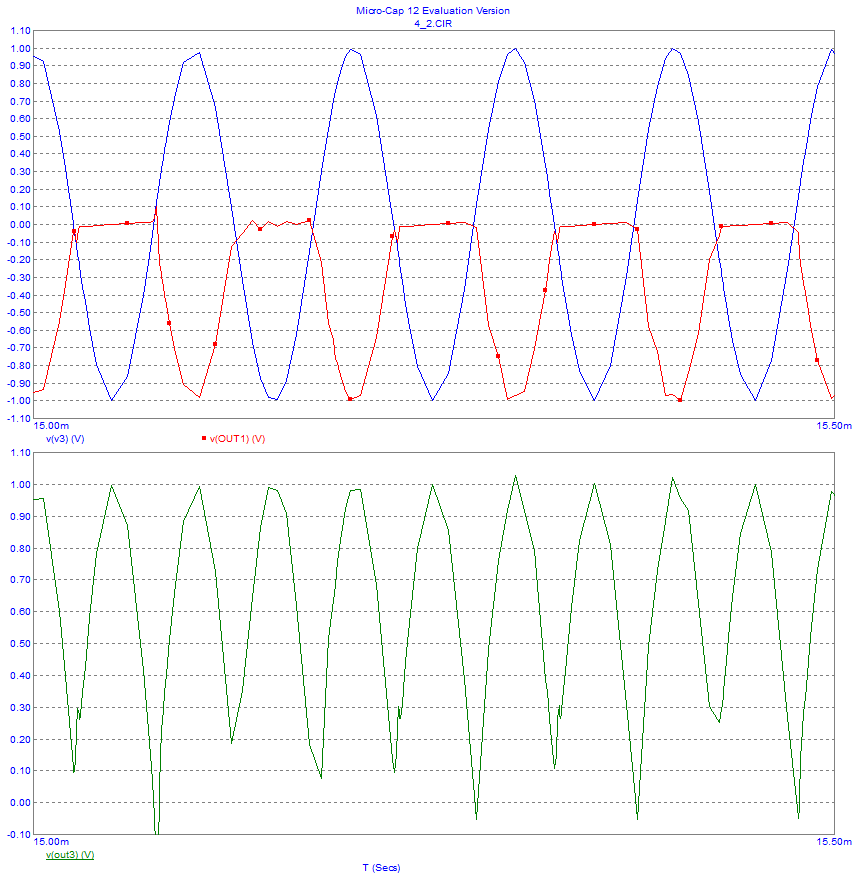
\includegraphics[width=0.7\textwidth]{microcap/2-transient-10khz-1v.png}
    \caption{Zapojení b) -- časová závislost napětí na výstupech obou OZ na vstupním napětí, nejvyšší frekvence, při které uspokojivě usměrňuje, \(f=\qty{10}{\kilo\hertz}, U_M=\qty{1}{\volt}\).}
    \label{fig:microcap/.png}
\end{figure}

\begin{figure}[h!]
    \centering
    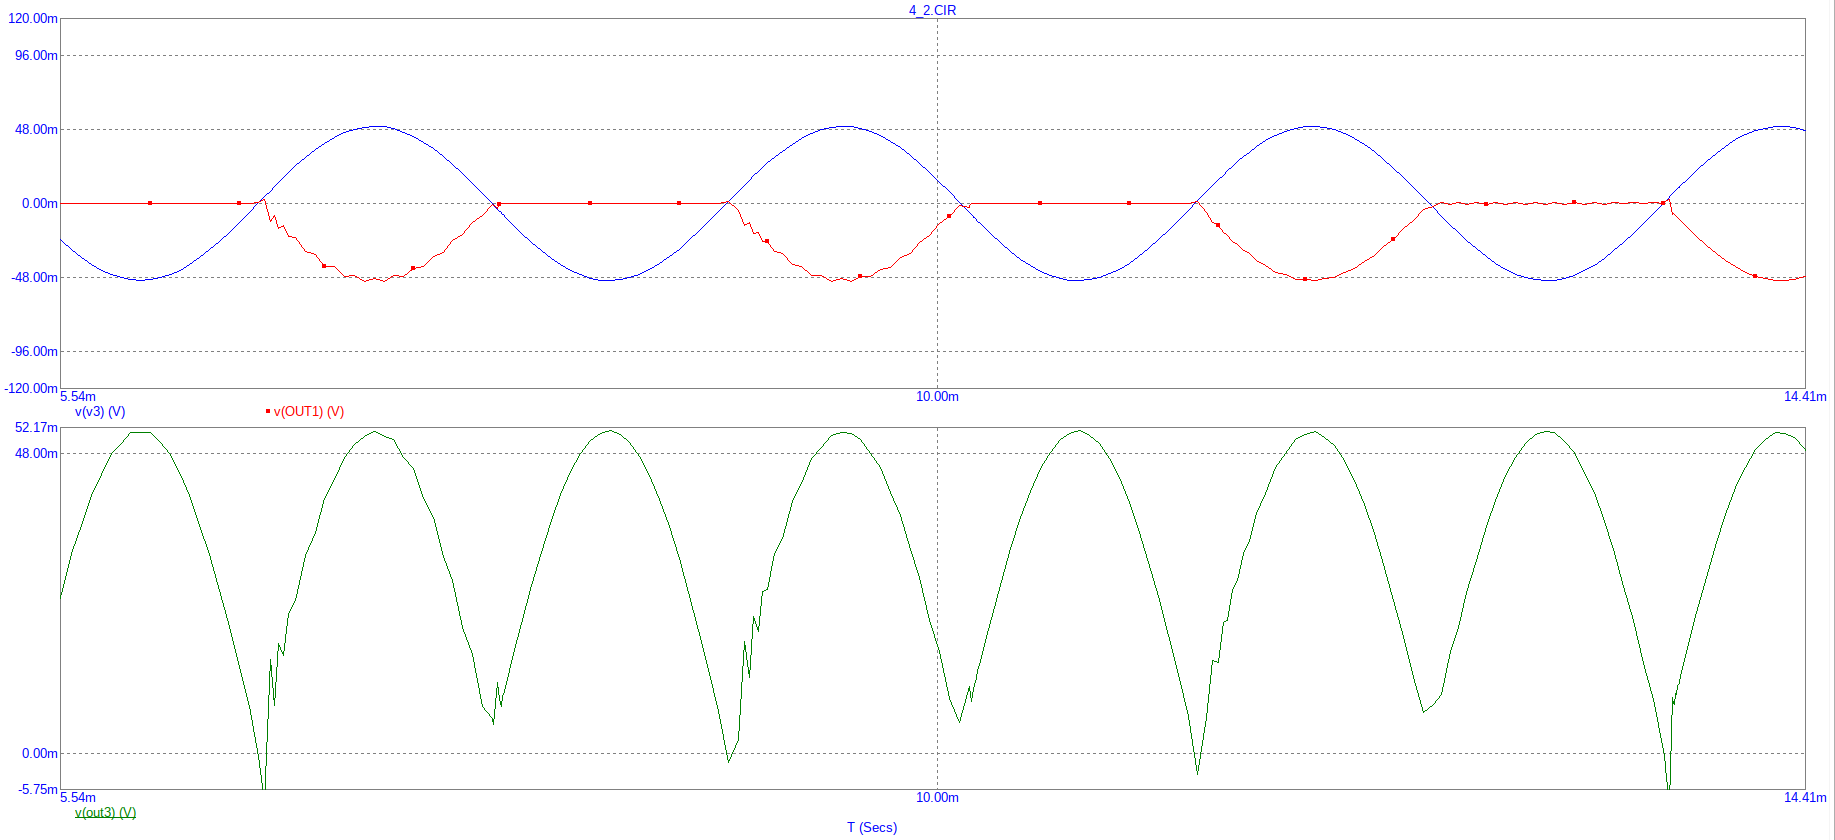
\includegraphics[width=0.7\textwidth]{microcap/2-transient-420hz-0.05v.png}
    \caption{Zapojení b) -- časová závislost napětí na výstupech obou OZ na vstupním napětí, nejnižší amplituda, při které uspokojivě usměrňuje, \(f=\qty{420}{\hertz}, U_M=\qty{50}{\milli\volt}\).}
    \label{fig:microcap/.png}
\end{figure}

\begin{figure}[h!]
    \centering
    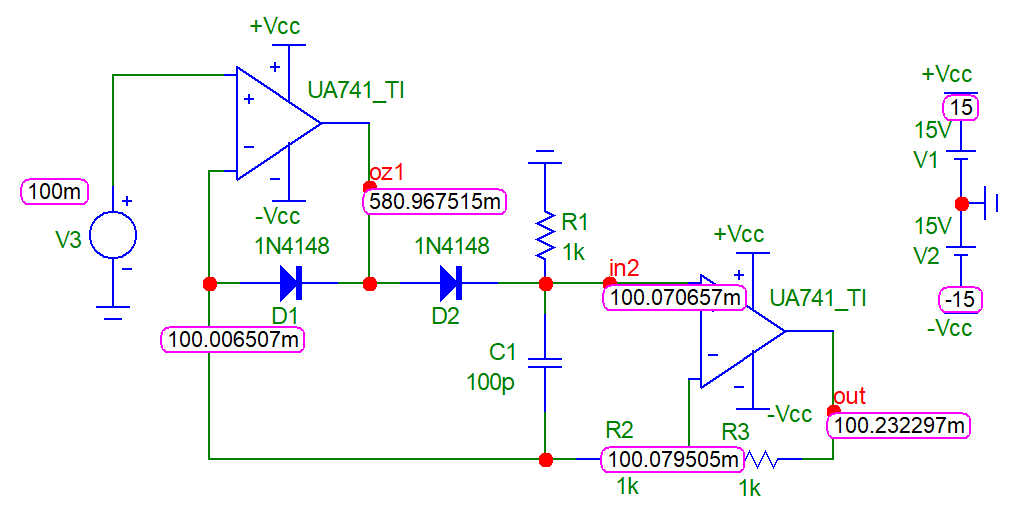
\includegraphics[width=0.8\textwidth]{microcap/3-dcbod.png}
    \caption{Zapojení c) -- stejnosměrný prac. bod při kladném napětí na vstupu, na výstupu kladné napětí.}
    \label{fig:microcap/.png}
\end{figure}

\begin{figure}[h!]
    \centering
    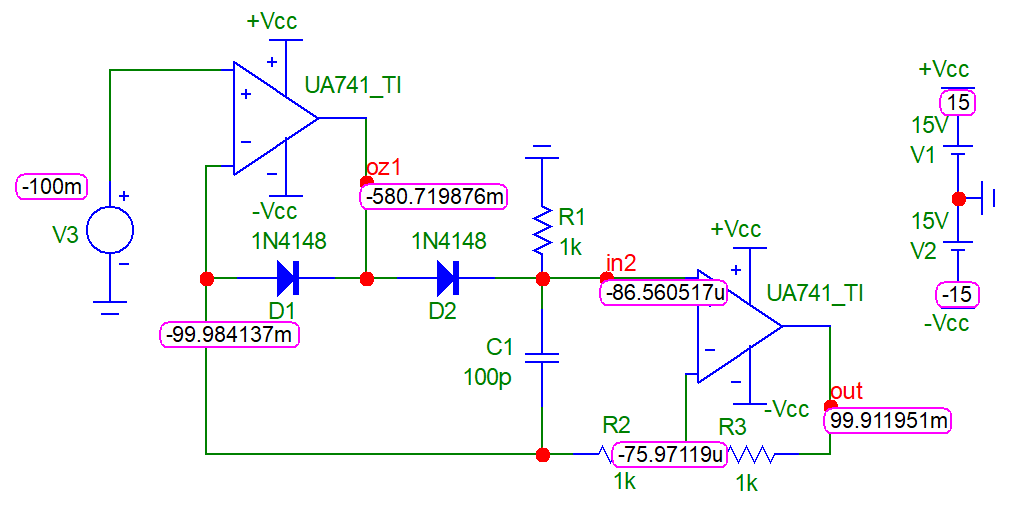
\includegraphics[width=0.8\textwidth]{microcap/3-dcbod2.png}
    \caption{Zapojení c) -- stejnosměrný prac. bod při záporném napětí na vstupu, na výstupu kladné napětí.}
    \label{fig:microcap/.png}
\end{figure}

\begin{figure}[h!]
    \centering
    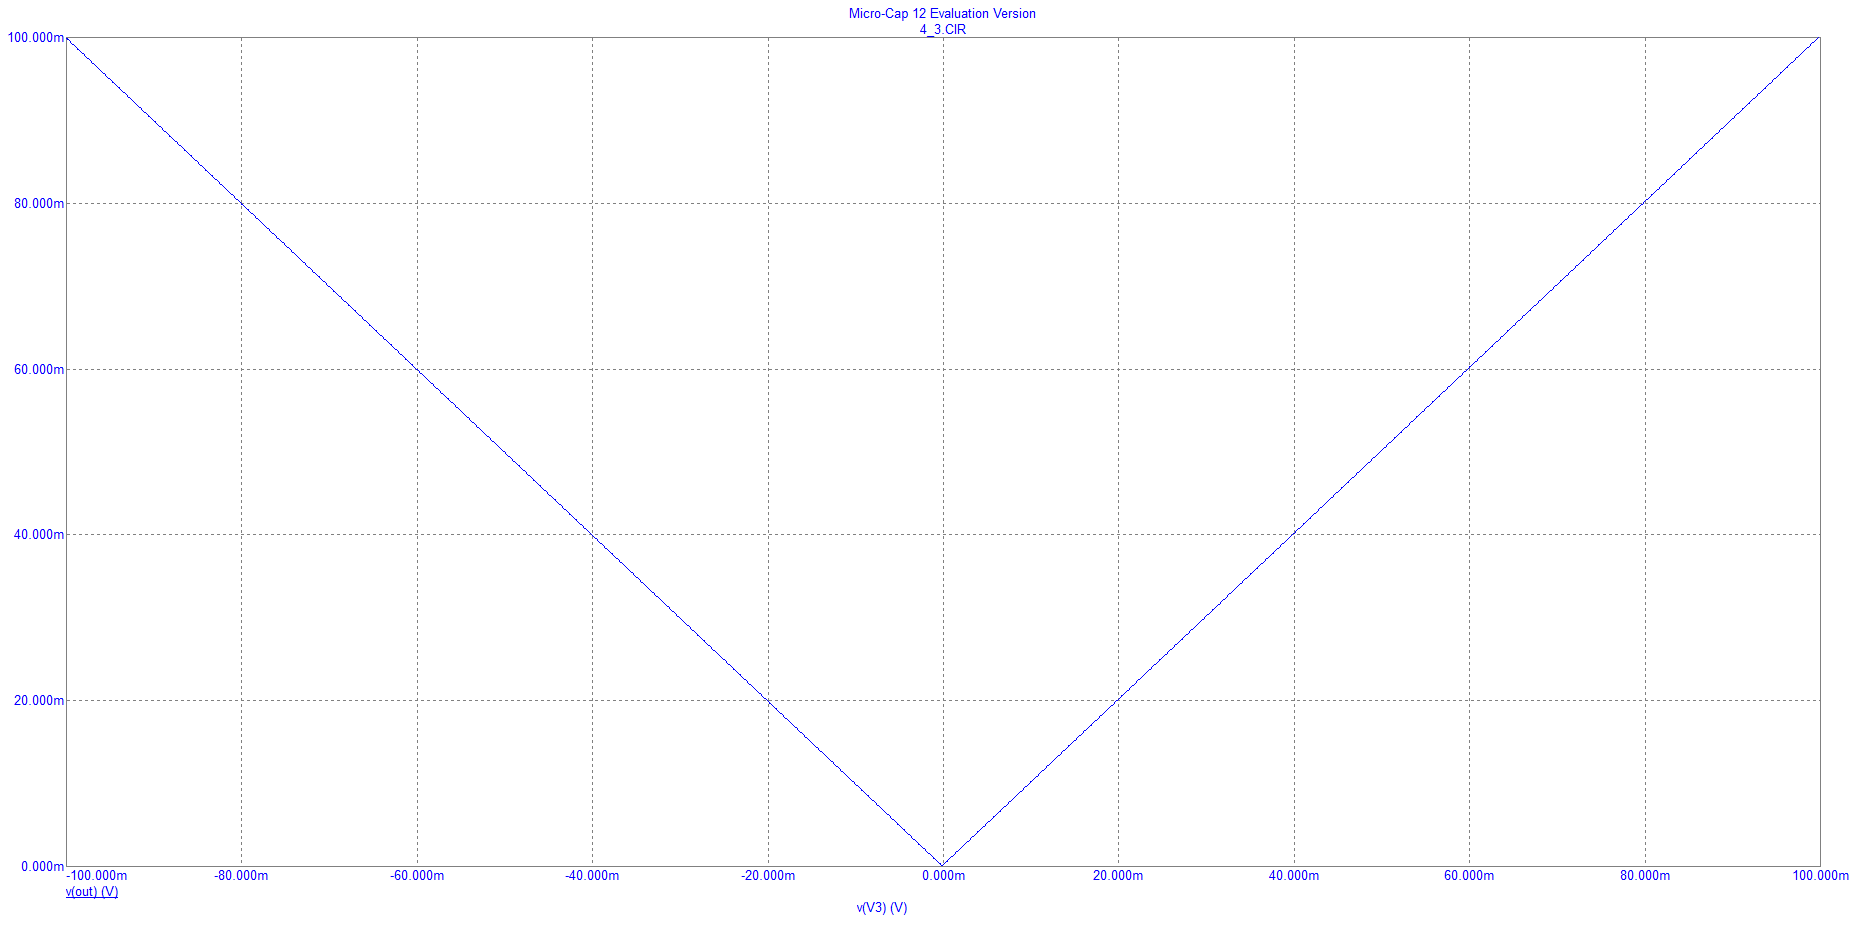
\includegraphics[width=0.8\textwidth]{microcap/3-dcprevodni.png}
    \caption{Zapojení c) -- stejnosměrná převodní charakteristika.}
    \label{fig:microcap/.png}
\end{figure}

\begin{figure}[h!]
    \centering
    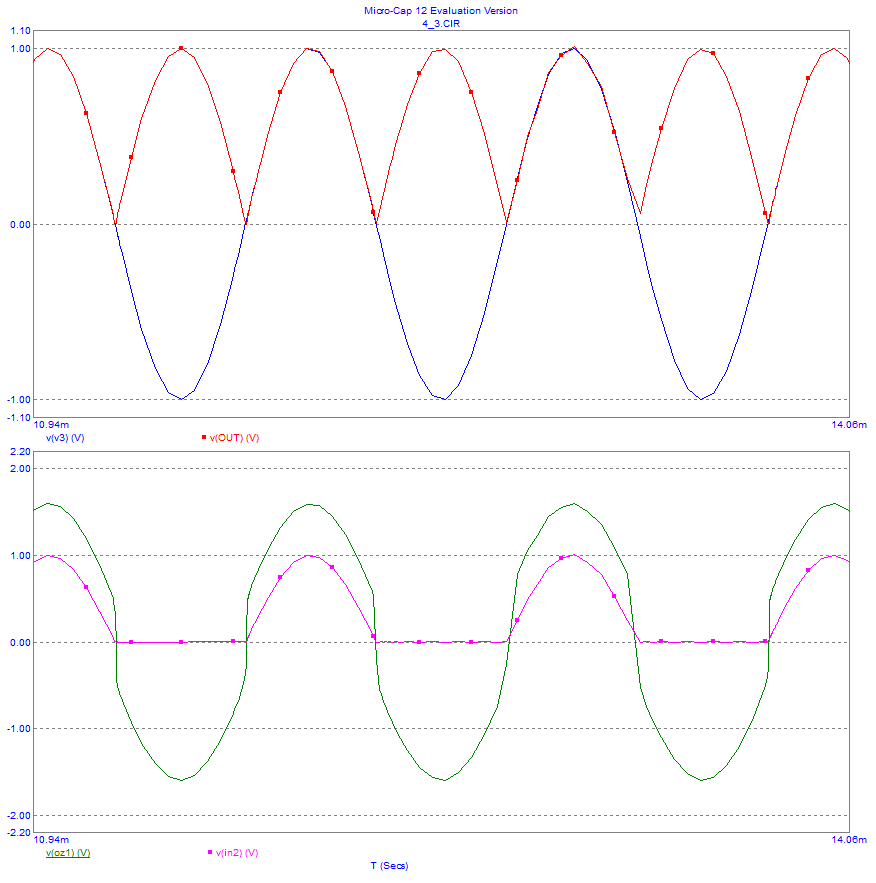
\includegraphics[width=0.66\textwidth]{microcap/3-transient-1khz-1v.png}
    \caption{Zapojení c) -- časová závislost napětí na výstupech obou OZ na vstupním napětí, jednocestné a dvoucestné usměrnění, \(f=\qty{1}{\kilo\hertz}, U_M=\qty{1}{\volt}\).}
    \label{fig:microcap/.png}
\end{figure}

\begin{figure}[h!]
    \centering
    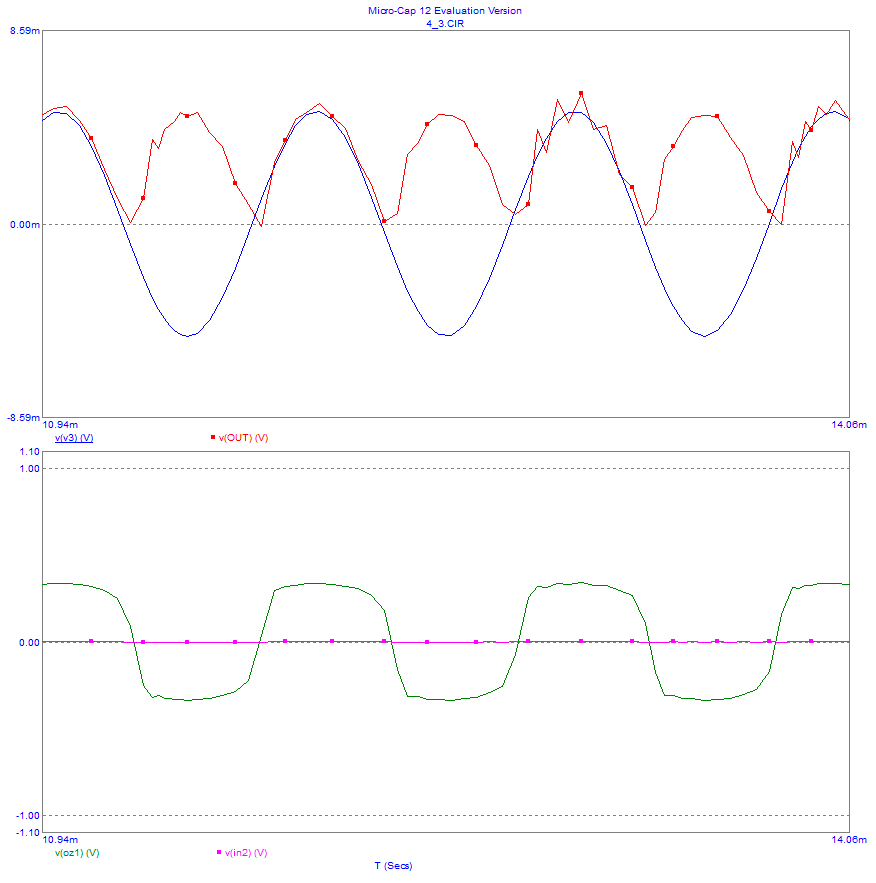
\includegraphics[width=0.66\textwidth]{microcap/3-transient-1khz-5mv.png}
    \caption{Zapojení c) -- časová závislost napětí na výstupech obou OZ na vstupním napětí, nejnižší amplituda, při které uspokojivě usměrňuje, \(f=\qty{1}{\kilo\hertz}, U_M=\qty{5}{\milli\volt}\).}
    \label{fig:microcap/.png}
\end{figure}

% \begin{figure}[h!]
%     \centering
%     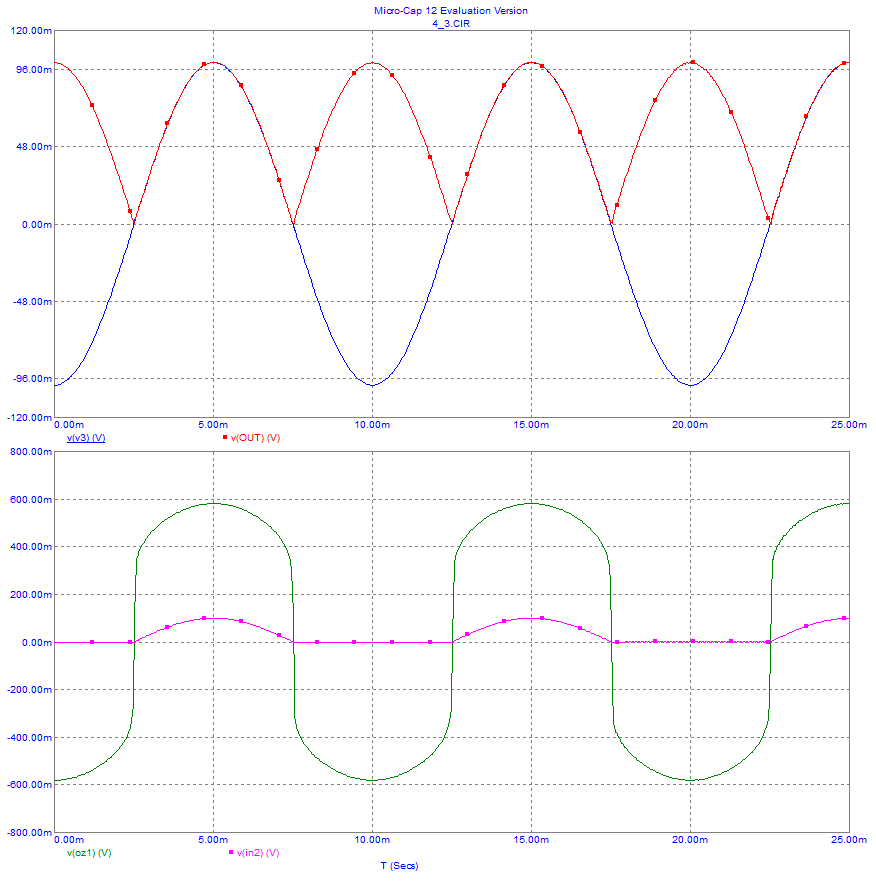
\includegraphics[width=0.8\textwidth]{microcap/3-transient-100hz-0.1v.png}
%     \caption{microcap/.png}
%     \label{fig:microcap/.png}
% \end{figure}

\begin{figure}[h!]
    \centering
    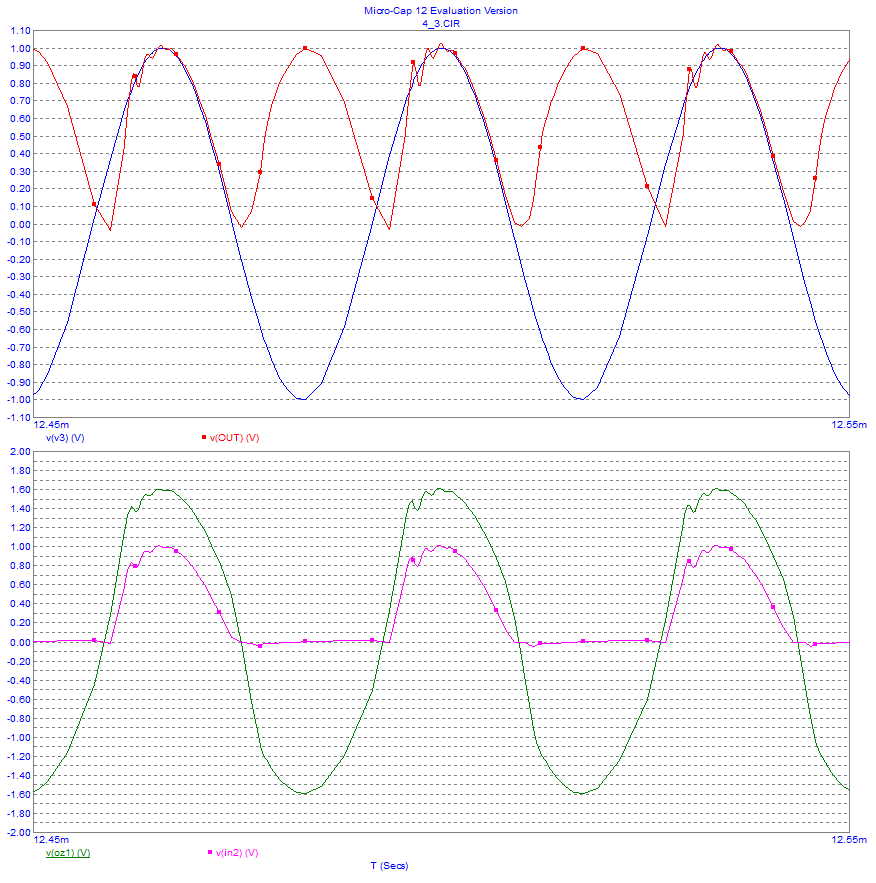
\includegraphics[width=0.8\textwidth]{microcap/3-transient-30khz-1v.png}
    \caption{Zapojení c) -- časová závislost napětí na výstupech obou OZ na vstupním napětí, nejvyšší frekvence, při které uspokojivě usměrňuje, \(f=\qty{30}{\kilo\hertz}, U_M=\qty{1}{\volt}\).}
    \label{fig:microcap/.png}
\end{figure}


%		
%	\clearpage

\section{Zpracování měřených hodnot}

\begin{table}[h!]
	\centering
	\def\arraystretch{1.4}
	\begin{tabular}{ |l|l|l|l|l|l|l|l| }
		\hline
		$ I_{in} \ [\unit{\ampere}] $ & 
		$ U_{in} \ [\unit{\volt}] $ & 
		$ P_{in} \ [\unit{\watt}] $ &
		$ \theta\ [\unit{\degreeCelsius}] $ &  
		$ I_{out} \ [\unit{\milli\ampere}] $ &
		$ U_{out} \ [\unit{\volt}] $ &
		$ P_{out} \ [\unit{\milli\watt}] $ &
		$ \eta\ [\unit{\percent}] $
		\DTLforeach{prvni}{\A=I1,\B=U1,\C=P1,\D=t,\E=I2,\F=U2, \G=P2, \H=etha}
		{\DTLiffirstrow{\\ \hline \hline}{\\ \hline} %
			\num[round-mode=places,round-precision=2]{\A} &
			\num[round-mode=places,round-precision=2]{\B} &
			\num[round-mode=places,round-precision=2]{\C} &
			\num[round-mode=places,round-precision=2]{\D} &
			\num[round-mode=places,round-precision=2]{\fpeval{\E * 1000}} &
			\num[round-mode=places,round-precision=2]{\F} &
			\num[round-mode=places,round-precision=2]{\fpeval{\G *1000}} &
			\num[scientific-notation = true,round-mode=places,round-precision=2]{\H}} \\ \hline
	\end{tabular}
	\caption{\label{tab:tabulka-vykon} Tabulka naměřených a vypočtených hodnot.}
\end{table}


\[
	P=U\cdot I 
\]
\[
	\eta = P_{out}/P_{in}  
\]

\begin{figure*}[h!]
	\begin{tikzpicture}
		\centering
		\begin{axis}
			[
			xlabel={\( P_{in}\ [\unit{\watt}]\)},
			ylabel={\( \theta\ [\unit{\degreeCelsius}]\)},
			axis y line*=left, % dve y osy
			width=1\textwidth,
			height = 0.5\textwidth,
			legend pos=north west,
			xmin=70,
			% ymin=,
			xmax=180,
			ymax=380
			]

			\addplot[mark=x, thick, blue, only marks, mark size=3pt] table [skip first n=2, x=P1, y=t, col sep=comma] {data/prvni-cast.csv};
			
			\addlegendentry{Teplota výměníku tepla}
			
		\end{axis}   
	 
		
		% Second y axis 
		\begin{axis}
			[
			ylabel={\(\eta\ [\unit{\percent}]\)},
			axis x line=none,
			axis y line*=right,
			width=1\textwidth,
			height = 0.5\textwidth,
			legend pos=north east,
			xmin=70,
			ymin=2.5e-4,
			xmax=180,
			ymax=7e-4
			]

			\addplot[mark= +, thick, red, only marks, mark size=3pt] table [skip first n=2, x=P1, y=etha, col sep=comma] {data/prvni-cast.csv};
			\addplot[samples=2,domain = 75:175,red,dashed, thin]{0.000489979-x*3.225855279410e-7};
			
			\addlegendentry{Účinnost motoru}
		
	\end{axis}
	    
	\end{tikzpicture}
	\caption{Závislost teploty výměníku tepla a účinnosti motoru na příkonu ohřívače.}
\end{figure*}


\begin{table}[h!]
	\centering
	\def\arraystretch{1.4}
	\begin{tabular}{ |c|c|c|c| }
		\hline
		Čas & 
		Měření 1 & 
		Měření 2 &
		Měření 3 \\ \hline
		$ t\ [\unit{\second}] $ & 
		$ \theta_{1}\ [\unit{\degreeCelsius}] $ & 
		$ \theta_{2}\ [\unit{\degreeCelsius}] $ & 
		$ \theta_{3}\ [\unit{\degreeCelsius}] $ 
		\DTLforeach{druha}{\A=cas,\B=tep1,\C=tep2,\D=tep3}
		{\DTLiffirstrow{\\ \hline \hline}{\\ \hline} %
			\A &
			\B &
			\C &
			\D } \\ \hline
	\end{tabular}
	\caption{\label{tab:tabulka-vykon} Tabulka naměřených časů pro různé teploty chladnutí.}
\end{table}


\begin{figure*}[h!]
	\begin{tikzpicture}
		\centering
		\begin{axis}
			[
			xlabel={\( t\ [\unit{\second}]\)},
			ylabel={\( \theta\ [\unit{\degreeCelsius}]\)},
			%axis y line*=left, % dve y osy
			width=1\textwidth,
			height = 0.5\textwidth,
			legend pos=north east,
%			xmin=0,
%			ymin=0,
%			xmax=100
%			ymax=100
			]

			\addplot[mark=x, mark options={solid}, thick, blue, solid, mark size=3pt] table [skip first n=2, x=cas, y=tep1, col sep=comma] {data/druha-cast.csv};
			\addlegendentry{Čerpadlo vypnuto}
			
			\addplot[mark=+, mark options={solid}, thick, red, dashed, mark size=3pt] table [skip first n=2, x=cas, y=tep2, col sep=comma] {data/druha-cast.csv};
			\addlegendentry{Čerpadlo zapnuto}

			% \addplot[mark=triangle, thick, green, only marks, mark size=3pt] table [skip first n=2, x=cas, y=tep3, col sep=comma] {data/druha-cast.csv};
			\addplot[mark=triangle, mark options={solid}, thick, green, dotted, mark size=3pt] table [skip first n=2, x=cas, y=tep3, col sep=comma] {data/druha-cast.csv};
			\addlegendentry{Čerpadlo zapnuto v opačném směru, od \SI{100}{\degreeCelsius}}
		\end{axis}   
	 
		    
	\end{tikzpicture}
	\caption{Časová závislost ochlazování výměníku pro různé módy tepelného čerpadla.}
\end{figure*}







		
	\clearpage
\section{Závěr}
	Podle struktury motoru jsme vyhodnotili, že se jedná nejspíše o modifikaci \(\gamma\).  	
	\\
	\\
	Nejprve jsme zkoumali motor v režimu generátoru - po dodání tepla se stirlingův motor začne otáčet a vytváří tak mechanickou práci, která je následně předána DC elektromotorku sloužícímu jako generátor. Protože se jedná o poměrně malý a nedokonalý model motoru, zaznamenali jsme vysoké výkyvy ve výkonu motoru, v některých momentech se dokonce zastavil. Snažili jsme se zaznamenat přibližnou průměrnou hodnotu, ale jak je vidět v Grafu 1, rozptyl měřených hodnot je dost vysoký. Z proložené přímky to vypadá, že účinost s rostoucím příkonem klesá, zřejmě kvůli větším tepelným ztrátám do okolí ohřívače.
	\\ \\
	Dále jsme stirlingův motor zapojili jako tepelné čerpadlo - tedy jsme elektromotor připojili ke zdroji napětí, dodával tedy do soustavy potřebnou mechanickou práci a stirlingův motor pohybem pístů přenášel teplo mezi ohřívačem a chladičem. 
	\\ \\ 
	Nejprve jsme měřili čas zchladnutí ohřívače bez pomoci čerpadla, následně se zapnutým čerpadlem. Z výchozí teploty \SI{300}{\degreeCelsius} na teplotu \SI{80}{\degreeCelsius} se při zapnutém čerpadle ohřívač ochladil o minutu rychleji. Z této teploty na výslednou teplotu \SI{40}{\degreeCelsius} pak bylo zapojení s čerpadlem o \SI{17}{\second} rychlejší. Tepelné čerpadlo tedy urychlilo přenos tepla z ohřívače do chladiče.
	\\ \\
	Při posledním měření se ohřívač nejprve chladil bez použití čerpadla do teploty \SI{100}{\degreeCelsius}, pak jsme zapli čerpadlo s opačnou polaritou elektromotorku (mělo by tedy chlazení zpomalit), na teplotu \SI{80}{\degreeCelsius} jsme se ale dostali stejně rychle jako v předchozím (urychleném) scénáři. Na finální teplotu jsme se dostali o celé dvě minuty dříve než v předchozím měření. 
	\\ \\
	Měření je tedy buďto krajně nespolehlivé a nebo byl špatný některý z našich předpokladů o fungování tepelného čerpadla.
\end{document}